% For easier proof-reading, use the single-column, double-spaced layout:
%\documentclass{cseminar}
% Final Paper use double-column, normal line spacing. Comment the line above and uncomment the following for the full paper
\documentclass[cameraready]{cseminar}

\usepackage{hyperref}
\usepackage[hyphenbreaks]{breakurl}

\begin{document}

%=========================================================

\title{Survey of ARM TrustZone applications}

\author{Pawel Sarbinowski\\
	\texttt{course:Seminar on Network Security}}
\maketitle

%=========================================================

\begin{abstract}

   ARM TrustZone security extensions were introduced almost a decade ago in the ARMv6 architecture and since then they have received a lot of attention as a security primitive in low-cost hardware. The main concept introduced in TrustZone is the separation of the CPU operating mode into a "secure" and "non-secure" mode. The two modes are isolated via hardware-based access control features without the need for a separate co-processor for the secure environment. Commonly, TrustZone technology is leveraged to run minimal pieces of software to which sensitive operations are delegates, while the regular operating system and applications are run in the non-secure mode.
   
Demands for trusted computing in commodity computing platforms, including handsets, tablets, wearable devices and even embedded systems, have stimulated the industry research. Innovative applications are also being explored increasingly by academia. Some of those include payment protection technology, digital rights management, BYOD (Bring Your Own Device) security enforcement, and a plethora of other security solutions.
   This paper surveys current applications of ARM TrustZone technology in both industry and academia. It also explores the ongoing standardization efforts involved in the domain, and identifies potential open research problems in the area.

\vspace{3mm}
\noindent KEYWORDS: ARM TrustZone, Trusted Execution, Integrity Monitoring, Linux, Virtualization, Mobile Security

\end{abstract}

%============================================================


\section{Introduction and Motivation}

In the past two decades the usage of mobile and embedded devices across all categories of computer ecosystems has increased rapidly. These devices, used by consumers or as infrastructure elements, are usually interconnected and create or contain vast amounts of information. At the same time, various stakeholders are striving to provide better security in the mobile ecosystem, motivated by several requirements.~\cite{untapped}~\cite{zone} Some of those include: 

\begin{itemize}

\item regulatory requirements, e.g. that the radio frequency parameters defined during manufacture are stored securely and remain unaltered. Recently, a bill in the state of California was passed that forces all mobile phones that are being sold to have a "kill switch" mechanism that will be able to shutdown and destroy the phones remotely in the event of theft or loss~\cite{killswitch}.

\item standardization requirements such as the mandate that the International Mobile Equipment Identifier (IMEI) remains unchanged. This is also important for uniquely identifying devices and dealing with thefts.

\item business requirements such as protection of digital content using Digital rights management (DRM) that is backed up by hardware security mechanisms or enforcement of phone operator subsidy locks to ensure that subsidized phones given to subscribers as part of a contract cannot be used with other mobile operators. Also remote attestation of the integrity of a client or employee computer might be necessary in cases of remote collaboration. This would ensure that the computing base used on the remote devices can be trusted and that the boot system and operating system have not been tampered with.

\item users security requirements that present the need for secure storage of various credentials and other private information (e.g. contacts) on mobile devices not only for login credentials but also for applications such as secure payments. Another scenario of interest can be performing integrity checks for anti-virus and anti-theft software to subsequently notify the user if something is altered.

\item developers interest in securing certain parts of their code that hold sensitive information (e.g. keys for remote API).

\end{itemize}

These raised security concerns have led to various system-level solutions employing hardware to run sensitive code or store private information in Trusted Execution Environments (TEEs). TEEs utilize specialized hardware to provide a secure, integrity protected environment for processing and storing information.

Currently, the TEE's functionality would not typically be available to third-parties, other than the Device manufacturers. OEMs take advantage of the TEE to protect resources (e.g. licensing metadata in the case of DRM) and functionality, such as crypto operations, from an adversary that has administrative control of the normal Operating System.
However, there are many use cases where third-party application, and not just the OEM, would also benefit from security features provided by a TEE. Examples of such applications are One-time Password generation for two-factor authentication, User Authentication mechanisms, Secure Mobile transactions for e-payments and even enforcement of Access Control for applications containing private data such as e-health apps. 
Alternative hardware architectures for implementing these kind of scenarios typically utilize a trusted co-processor (Trusted Platform Module or TPM) or hardware module (e.g. a SIM card) but a separate co-processor also leads to higher system costs and in some cases to a loss or difficulty in programmability.  

ARM TrustZone security extensions have been available for some time already, since the ARM11 Core which was released in 2002. They are available in the large majority of new mobile and embedded devices with ARM processors. TrustZone's main advantage, compared to other solutions that use a separate on-chip or off-chip co-processor,  is that it is inexpensive (i.e. no extra hardware chips are needed) and it takes advantage of the full processing power of the CPUs and not just a small subset of a slower secure chip. Both proprietary and open source TEE OS's and TEE applications are being built on top of TrustZone. At the moment,  there are ongoing efforts (noted later in \ref{standardization}) for easing the process of developing and debugging on top of TrustZone. This paper explores some of the implementations utilizing TrustZone from both academia and industry.

The structure of this survey is as follows: Section~\ref{background} provides an overview of TrustZone technology, presents the key concepts of the architecture and discusses some of the challenges in the field. Sections~\ref{userapps} and~\ref{osapps} present some existing relevant applications utilizing TrustZone and then \ref{relatedwork} and  \ref{standardization} discuss about related works and efforts to standardize the TrustZone API available for third party developers. Finally, Section~\ref{conclusion} provides some concluding remarks.

%============================================================

\section{Background}
\label{background}

Existing hardware security solutions can be separated to two groups: those that utilize separate trusted co-processors in a different chip either outside or inside the CPU die and those that utilize single-chip solutions where the hardware security is incorporated into the CPU architecture itself and there is no second co-processor. Secure co-processor architectures can be split furthermore based on the hardware they use to: Smartcards used in systems such as ATMs, SmartTVs and communication equipment(e.g. SIM cards); Trusted Platform Modules (TPM) which have a separate secure co-processor usually soldered on a PC board and are the primary means of providing standardized trusted computing features to PCs; and Hardware Security Modules (HSM) that may have more than one cryptoprocessors inside and offer multiple levels of security not only against software attacks but also against physical attacks.

Some of the double-chip CPU architectures include: Intel TXT, which uses a TPM and measures the integrity of software and platform components (i.e. code, data structures, configuration files and more) in order to allow management applications to make trust decisions correspondingly, AMD PSP (Platform Security Processor), which uses a dedicated co-processor that features ARM TrustZone technology to guarantee features like secure boot, trusted execution and more.

Examples of some platforms having a single chip are: AEGIS~\cite{aegis}, that utilizes memory integrity verification, encryption/decryption of off-chip memory and a secure context manager; XOM~\cite{xom} (eXecute Only Memory), where the processor is equipped with a private key, known only to the processor manufacturer, and the corresponding public key is published. Hence, anyone can encrypt the software by using the public key but only the processor having the corresponding private key can decrypt and execute the software. All software is stored encrypted in memory when it is executed; Intel SGX (Software Guard Extensions)\cite{intelsgx}, which constitutes a set of new CPU instructions that can be used by applications to specify protected regions of code and data referred to as enclaves. An enclave is a protected area in the application's address space, which provides confidentiality and assures integrity even in the presence of privileged malware. Accesses to the enclave memory area from any software not resident in the enclave are prevented; and finally ARMs' TrustZone platform.

\begin{figure}[t]
  \begin{center}
    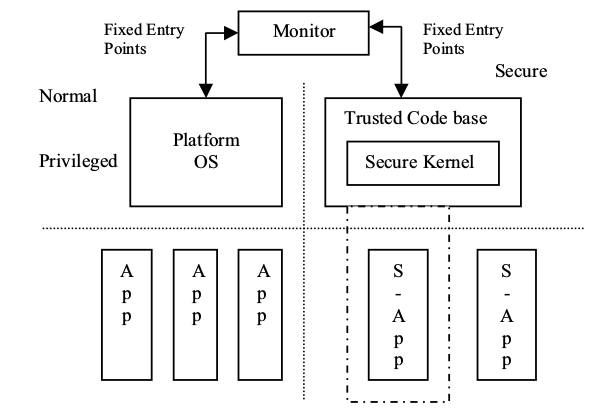
\includegraphics[width=.5\textwidth]{figures/trustzone_arch}
    \caption{TrustZone architecture\cite{epassdrm}}
    \label{fig:trustzone_arch}
  \end{center}
\end{figure}

\subsection{ARM TrustZone}
\label{armtrustzone}

The ARM TrustZone architecture (Fig.~\ref{fig:trustzone_arch}) serves as a much more flexible single-chip alternative, with a fully functioning CPU whose secure component is freely programmable, compared to the double-chip solutions that have a fixed programming interface and usually feature set for secure applications to use. Programming a TEE on top of a double-chip TPM or HSM is also feasible but there are drawbacks in terms of performance since the secure co-processor is a more limited chip due to its cost.
TrustZone introduces the concept of two logical processing modes for the ARM CPU, referred to as "secure world" and "normal world" mode. Each mode is isolated via hardware-based access control features from the other one. Typically, TrustZone technology is leveraged to run small, security-specialized portions of code in the secure world mode, whereas the conventional operating system and applications are run in the normal world mode.
The distinction between the worlds is implemented in hardware thus prevailing software protection rings between user-level and kernel-level code are not affected. The operating system does not have to be aware of the two cpu modes for the applications to utilize them. The hardware separation is also propagated over the system bus to peripheral devices, memory controllers and cpu registers. Thus, when secure mode is active, the software running on the CPU has a view of the whole system that is isolated from the software that is running in non-secure mode.

The main benefit of this approach is the minimal loss in processing power of the secure cpu component (which is now the same cpu) and the extensible functionality a programmer can implement on the cpu instead of the hard-wired actions previously found on TPMs. To transition between the two worlds a special \textit{Secure Configuration Register} (SCR) is used. Specifically, the Non-Secure bit in the register (SCR.NS) is set to 1 to transition from the secure to the non-secure world. Code running in normal mode cannot directly change the NS bit, therefore to enter to the secure mode again, a set of calls is defined and includes secure monitor calls, interrupts and external memory system aborts. Secure monitor calls are handled in the secure world and act as a sort of cross-world system call.

For completeness we will also define some additional terms such as: Rich Execution Environment (REE) is the full-feature operating system such as Linux, Windows, OS X, Android or iOS; TEE OS is the operating system running in the secure world and is usually comprised of a micro-kernel, a memory management unit and code implementing an API for Client/Trusted apps; TEE is a superset of that and  essentially includes all the functionality (in hardware and software) that is necessary for the controlled isolation of secure apps from the REE; Trusted Application (TA) is an application that is running inside a TEE and provides certain functionality to Client Applications; finally Client Application (CA) is an application running in the normal world (REE) that accesses a TA's functionality or offloads a security critical part of it's own to a running TA.

The main features of the TrustZone platform can be split into: Boot Integrity, Secure Storage, Device Identification, Isolated Execution, Device Authentication and an API to access the TZ features. A quick overview of these components follows:

\textbf{Boot Integrity} - Acts as a building component for the security of the entire system. Verifies the integrity of the software at each stage of the boot (bios firmware, bootloader, operating system). The boot code's signature hash is checked against a securely stored hash that was signed by the device manufacturer. The device manufacturer's public key is used to decrypt the signature and to compare the two hashes. The comparison of the hashes continues for each subsequent boot stage and if they at some point differ, the device stops the boot (in the case of secure boot) or stores the different measurements for later usage by the OS or applications (in the case of authenticated boot). 

\textbf{Secure Storage} - Uses cryptography to preserve the confidentiality and integrity of application data. Usually the encrypted data is stored in other insecure peripherals (e.g. a hard disk) but it is encrypted with a key that is stored inside the secure non-volatile memory of the CPU. All the cryptographic methods are also executed in the context of the secure world.

\textbf{Device Identification} - Uses the secure storage feature to verify and preserve multiple unique identifiers for each device. A base identity is defined and certified by the device manufacturer, which stores it in the secure non-volatile memory. This base identity can then be used to verify and sign new assigned identities that can be used for e.g. e-ticketing applications.

\textbf{Isolated Execution} - Runs trusted applications inside the secure world separated from each other and from the normal world. It also guarantees that any code and data running in the secure world is protected at run-time from access even from privileged code running in the normal operating system. A minimal TEE Operating system is used to manage Trusted applications running in the secure world as well as communication with them. Trusted applications that intend to run in the secure environment will have to be signed by the device manufacturer.

\textbf{Device Authentication} - Verifies the integrity of the system to third parties that need attestation. In this case, the system's state (O.S. running, boot software signature and trusted application) is signed with a device specific key known to the device manufacturer before-hand. The signed device authentication can then be verified by a third party by using the public key of the manufacturer that signs a pre-defined set of known system configurations (OS, boot code, apps etc) that are acceptable for the device, thus proving the integrity of the system.

\textbf{API} - The TEE operating system, running in the secure world, provides an programming interface for communication between Client Applications (CAs) in the "insecure" OS and Trusted Applications in the TEE, and even between Trusted Applications in the TEE. In the latter case, the isolation is provided by privileged mode code part of the TEE OS, not distinct hardware features.

%-----------------------------------

\subsection{TEE implementations}
\label{teeoss}

The ARM TrustZone extensions~\cite{trustzonewhitepaper} define mainly the hardware architecture necessary for a secure computing component. To develop an application on top of those extensions a TEE is necessary. Although ARM provides some basic examples~\cite{trustzoneexample} of how to utilize the TZ security monitor to develop simple applications on top of TrustZone, in the long-term a more complex dedicated TEE OS running in the secure world will be a more robust solution capable of managing several Trusted Applications at the same time. Several proprietary TEE Operating Systems are already built on top of the TrustZone architecture to provide the necessary functionality and management of Trusted Applications. 

Mobicore OS was initially developed by a company called Giesecke \& Devrient (G\&D), which together with the ARM Secure Services Division and Trusted Logic Mobility (TLM)  established Trustonic~\cite{trustonic}. Now, Trustonic provides both a (GP compliant~\ref{standardization} ) TEE operating system and a TEE Directory. TEE Directory is a framework for remote deployment and management of Trusted Applications built on top of Trustonic's TEE. It adheres to the GP remote management protocol standard. Trustonic provides an SDK for its TEE to developers (after registration) and acts as a Trusted Service Manager for the Trusted Apps that are deployed.

Qualcomm has also implemented a proprietary TEE OS of it's own called Qualcomm Secure Execution Environment (QSEE)~\cite{qualcommqsee} on top of TrustZone as provided in it's S4 Snapdragon 8XXX processor series. Besides the TEE, Qualcomm's environment also provides several proprietary Trusted Applications such as: StudioAccess for DRM in media streamed by partners among which are Amazon, Hulu, Netflix and more; Enterprise and BYOD for securing corporate data on employees devices with device-unique crypto keys; SafeSwitch that acts as a remote kill switch in case of theft; Authentication by using biometrics based on Fast IDentity Online (FIDO) standard. Finally QSEE provides a TA that acts as a hardware back-end for Android's Keystore API. 

Finally Solacia has also implemented SecuriTEE OS~\cite{solaciatee} as a proprietary TEE that adheres to the GlobalPlatform standards and is mostly used for secure payments and content protection.

All the aforementioned implementations are closed source, require licensing fees to use or develop on them and thus restrict the development of TEE Applications by more programmers. 

%============================================================

\section{Applications utilizing TrustZone}
\label{userapps}

Existing applications based purely on TrustZone-provided features (i.e. trusted applications built on top of the TEE OS) are described in the following papers[\cite{epassdrm},\cite{designembedded},\cite{privacytrustzone},\cite{experimenting},\cite{twofactorauth}].

Motivated by the increase in both mobile device usage and in the ease of digital content distribution in the past decades Hussin.~et.~al.(\cite{epassdrm}), examines the usage of TrustZone for secure storage and enforcing of DRM policies. It utilizes an existing DRM distribution model found in Symbian OS. In this model, however, DRM metadata files and vital application data (such as media files, game levels, data controlling the application logic) are stored in the TrustZone-based secure storage. Furthermore, the DRM License Manager, which is in charge of regulating application execution through licenses and protecting application data, is run inside the secure world to ensure integrity of execution. The authors also propose an E-Pass application based on this DRM model, where the ticket issuer and the user will share a signed electronic pass. The pass will be stored transparently in the user's secure hardware and will resist tampering.
 
A platform, backed by TrustZone, for anonymous electronic payments is presented by Picker and Slamanig~(\cite{privacytrustzone}) where they try to unify the convenience of electronic payments with the anonymity of cash. Traditionally in electronic payments, a user first purchases electronic credit via some sort of e-banking and then he/she uses the credit on the provider's services (e.g. in the context of a transport payment system). To avoid the linking of users' banking accounts to their transport information the authors introduce signed electronic tokens that a user can buy anonymously with cash. The tokens are in the form of printed QR-codes that a user can scan with his smartphone. The signed token is then stored in the TZ secure storage to preserve privacy even in the event of the phone loss. The transport provider will also have to keep a corresponding list of the tokens issued for usage but there is no need to keep any type of personal information for the users, thus preserving their private information. The sensitive computations and storage would run as a Trusted Application (Trustlet) in the context of TrustZone.

Rijswijk-Deij.~et.~al(\cite{twofactorauth}) - investigate the possibility of using a device having TrustZone capabilities to implement One Time Passwords (OTP) for two-factor authentication with a comparable level of security. To allow the comparison, a conceptual model of user interaction with OTP applications is introduced and studied. The model assumes there is a trusted path to the display, all user input passes through a TrustZone secure peripheral bus and that the Memory Management Unit support protected memory separation between the secure and the normal world. They show that a trusted path can exist between user input and display of OTP credentials, albeit with two disadvantages. First, the chip manufacturer is the external entity that must be trusted so that the system can work, and, second, that TZ does not come with a dedicated software implementation by itself, complicating its usage by developers.

%-----------------------------------

\section{REE OS Hardening}
\label{osapps}

Research applications that effectively build another abstraction layer on top of the TEE OS are presented below. They aim mostly at creating a middle layer that either secures certain procedures transparently or provides a much easier to use API for applications to do so.

TrustZone-based Real-time Kernel Protection (TZ-RKP)~\cite{hypervision} is an approach aiming to provide enhanced security to the Operating System kernel by transferring its security monitor to the TrustZone secure world. Consequently the security monitor that handles all access control is protected from attacks originating in the normal world where the rest of the kernel is running. TZ-RKP transfers the control over privileged system functions to the secure world where each access request is inspected before being granted. Examples of such malicious actions can be requesting for system sensitive data, hiding malicious processes or escalating the privileges of a malicious app. Existing hypervisor solutions achieve the same goal but are themselves also prone to attacks from processes running in the normal world. The target kernel runs in normal world while TZ-RKP, containing the security monitor, runs in the secure world. By running the security critical part of the kernel in the hardware backed secure world, TZ-RKP achieves a compromise between security and usability and since it is already deployed in Samsung Galaxy devises it is a tested and feasible approach. To guide the flow of code execution through the access monitor and memory management unit, residing in the secure world, TZ-RKP utilizes hooks in the kernel. This provides full control over the memory management of the normal-world kernel as well as live interception and monitoring of critical events that can be denied if they negatively impact the security of the system. To further ensure that the kernel hooks used are not altered or bypassed by a malicious process, TZ-RKP also: maps the memory containing the kernel code as read-only; defines the memory area containing dynamically allocated kernel data (such as virtual-to-physical memory translation tables) as read/write only by the kernel code and as non-executable; allows only trusted applications that are signed, verified and inspected to run in the TEE.  Extensive testing confirmed TZ-RKP's effectiveness and benchmarks performed showed that the overhead of this system is minimal  and ranges between 0.2\% and 7\%.

A security enhancing framework is introduced by Zu.~et.~al.(\cite{designembedded}) designed for embedded systems running Linux. This development is motivated by the increase in usage of embedded systems in pervasive computer environments (e.g. networking stacks, Internet of Things devices, instruments for automation and devices used in aeronautic research). The proposed framework includes a Linux Security Module that hooks on the Linux kernel and enforces additional access policies based on security models such as Bell-La Padula and the Domain and Type Enforcement model. To ensure that the security policies cannot be tampered with without authorization, the framework is mainly implemented as a Trusted application running in the secure world of TrustZone and provides an API for the LSM hooks of the kernel. This acts as an extra layer of Mandatory Access Control similar to the way modules like SELinux, AppArmor and Smack work but since it is backed on the TZ hardware, it is significantly harder for attackers to bypass without physical access.
 
A virtualization platform design to secure embedded and mobile systems is proposed by Johaness Winter~(\cite{trusted}). The core idea of it is to split insecure software into isolated user-space VMs that communicate with secure-world trusted engines. These are managed by a Linux based kernel running in the secure world that enforces MAC (mandatory access control) and isolated execution with SELinux policies. Each of these Trusted engines has a properly defined interface for communicating with other trusted engines. The isolation of the Trusted Engines is based on the features TrustZone offers i.e. secure peripherals cannot be accessed by non-secure software and non-secure software cannot access secure memory without authorization from the secure-world. The proposed architecture handles all the low-level details, such as dispatching secure monitor calls, and enforces restrictions on the resource usage of the non-secure mode software code. 
The platform uses a secure boot loader that authenticates the secure world linux kernel image and measures it. This measurement is then compares to a Reference Integrity Metric (RIM) certificate that is attached to the kernel image. Only if the RIM certificate matches to the integrity measurements taken, will the boot continue and control will be handed to the Operating system running in the non-secure world. 
To communicate with secure code any secure monitor call that is invoked by non-secure code is handled by the user-space VM supervisor. This VM supervisor acts as a middle layer between non-secure apps and secure-world Linux kernel, thus minimizing the amount of processing the secure kernel has to do. Eventually the authors plan to integrate the TrustZone based virtualization framework with the KVM virtualization framework found in Linux kernels.

A Trusted Language Runtime (TLR) is proposed, implemented and evaluated by Santos.~et.~al.~(\cite{tlrms}). The TLR aims to act as a mechanism for isolating security-sensitive  application logic from the rest of the application, the Operating system as well as other applications. It is based on a lighter .NET Micro runtime Framework (NETMF) designed for embedded devices, thus managing to keep the trusted computing base code reasonably small. 
The framework handles low level details some of which are secure memory or cpu resource sharing, interrupt handling across domains and coordination of the execution flow of the apps between secure and non-secure worlds. By obscuring these details the framework allows developers to easily split their security-sensitive code into classes that transparently run in a trusted environment, isolated from the rest of the app, the operating system and from other Trusted applications (by using TrustZone features) and in a development framework (.NET) which they are already familiar with. Figure~\ref{fig:netmf_arch} provides a better overview of the framework.

\begin{figure}[t]
  \begin{center}
    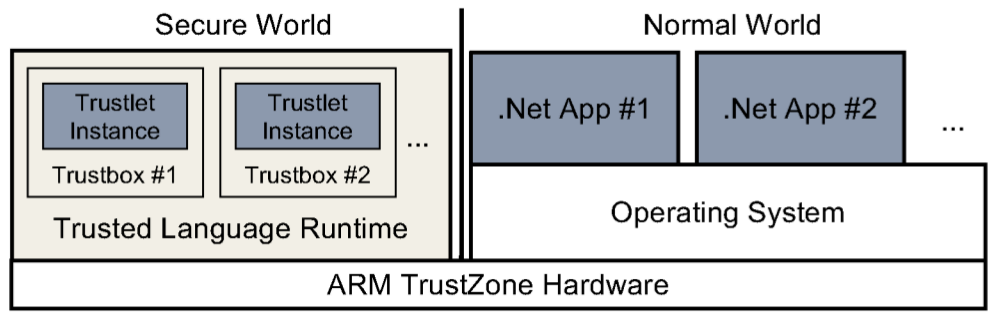
\includegraphics[width=.5\textwidth]{figures/netmf_arch}
    \caption{TLR high-level architecture\cite{trusted}}
    \label{fig:netmf_arch}
  \end{center}
\end{figure}

To maintain a small TCB certain restrictions were introduced to the runtime. Code that is running on the Trusted Instance of the runtime (in the secure world) can only perform computations or encrypt/decrypt data associated with trusted classes. It cannot access peripherals. Otherwise the TLR would have to include drivers to access them which would increase the codebase significantly. Sample use cases of apps utilizing the TLR secure features include One-time Password generators, User authentication and Secure Mobile Transactions (both based on a challenge-response protocol running on trustlets) and enforcement of access control to secure data used or collected by e.g. e-health applications.

%-----------------------------------

\section{Related Work}
\label{relatedwork}

Because very little work had been done on open source software for TrustZone systems Johannes Winter~(\cite{experimenting}) explores system-level development on cost-efficient arm devices, particularly in a classroom environment. The goal is to utilize this knowledge to teach TEE programming in classrooms. Obtaining such knowledge had been troublesome since most TrustZone enabled board manufacturers either do not provide any technical support or they do only after signing a non-disclosure agreement which complicates matters significantly for academics. In the paper the authors: analyze the TrustZone platform of a specific ARM board, discuss the problems that arose while developing a micro-kernel prototype that would run in the secure world, present methods to test the basic TrustZone functionality of a board as well as a simple architecture for initial development of apps running in normal mode, and, finally, demonstrate the development of a secure boot-code while also analyzing the board's internal boot ROM structure.

Motivated by the lack of tools for debugging and developing TEE applications, McGillion.~et.~al.~(\cite{opentee}) introduce Open-TEE, a virtual TEE implemented entirely in software that emulates the TEE behavior as defined in the GP~\cite{gpspec} standards. By utilizing a software-based TEE emulator developers can avoid the cost of proprietary TEE software development kits or expensive hardware debugging tools, while at the same time taking advantage of already known, reliable debugging tools (such as GDB or LLDB) and development environments. Thus, after fully debugging and testing a Trusted Application, they will be able to compile it to any GP-compliant hardware TEE. To make it as simple as possible to deploy and work with, the framework was designed as a set of processes each implementing specific TEE operations (e.g. Trusted application, TA manager, TA launcher), thus the time and resource overhead to develop with Open-TEE is minimal. A small scale, but extensive, user study was also performed and showed positive results on the ease of use of Open-TEE and its benefit for the TEE development life-cycle. Open-TEE is freely available as open-source software under the Apache-V2 license.

Dan Rosenberg in his recent work covered a newly found vulnerability in the QSEE TEE software~\cite{qseevulnerability} which affects "all known Android devices that support TrustZone and utilize a Qualcomm Snapdragon SoC, with the exception of the Samsung Galaxy S5 and HTC One M8, which have been patched". The vulnerability is based on a bug in the bounds-checking the Secure Monitor performs on calls made by client apps. It allows a kernel-level application to write data to arbitrary secure-world memory, thus completely compromising any trusted application running in the TEE. Similar vulnerability research was also done in Azimuth Security in 2013 to exploit QSEE and bypass the Secure Bootloader in Motorola Devices.

%============================================================

\section{Standardization Efforts}
\label{standardization}

The restrictions of proprietary TEE implementations\ref{teeoss} and the difficulty in programming and debugging in them led to an increased need for both standardization of the TEE API and for open source implementations of TEE Operating Systems and developer tools. Steps already taken in that direction include the following.

"GlobalPlatform is a cross industry (Visa, MasterCard, NTT, ARM and others), non-profit association which identifies, develops and publishes specifications that promote the secure and inter-operable deployment and management of multiple applications on secure chip technology."~\cite{gpspec}. Around 2011, GP published specifications for the TEE client API (used by client applications running in the normal world), the TEE System Architecture and TEE Internal API (used for internal communication between the corresponding TEE parts running in secure and non-secure world). "GlobalPlatform has launched a TEE compliance program. This offers assurances to application and software developers and hardware manufacturers that a TEE product will perform in line with the GlobalPlatform standards and as intended. It also promotes market stability by providing a long-term, inter-operable and industry agreed framework that will evolve with technical requirements over time". Several TEEs including Mobicore OS, QSEE, SecuriTEE, OP-TEE and SierraTEE are already partially if not full GP compliant and therefore applications built on those specifications should be able to inter-operate between all platforms.

Besides the GP standardization effort, there have also been endeavors to create open source TEE operating systems as an alternative to the proprietary solutions mention in section~\ref{teeoss}.

Linaro~\cite{linarooptee} is an open organization focused on improving the security of Linux on ARM. Linaro along with STMicroelectronic developed OP-TEE, which is an Open Source TEE. It is based on a proprietary TEE solution that was Global Platform certified on some products in the past thus compliance with the GP standards is quite extended. Currently the secure TEE code runs on 32 bit only but there are plans to add support for 64 bit and to also upstream the OP-TEE kernel driver to the Linux kernel.

SierraTEE and SierraVisor~\cite{sierratee} are an open source TEE and hypervisor respectively that offer a comprehensive solution from secure boot to application management and are maintained by the Sierraware. They support applications in C, C++ and Java and are easy to integrate with android and other mobile platforms. They also have the option to use dedicated cores for normal and secure world OR share worlds between cores. It is a minimal TEE and offers protection against side channel attacks, supports several interrupt models, fast performance architecture, fast context switching and supports asynchronous IPC. It currently supports ARM11, Cortex-A9, and Cortex-A15 processors and is also available for 64bits.

%============================================================

\section{Conclusion}
\label{conclusion}

In this report we examined the research and product development done by academia and industry, for the ARM TrustZone architecture. Overall although the initial motivations for the research (i.e. securing the interests of all the stakeholders) remains we can observe a shift in how this research is performed. From mostly proprietary and not openly documented products to more and more solutions that are based on the GP standard and are even open source. The research area around TrustZone is positively active. And the reason is that even though TrustZone was partially marketed as a "silver bullet" for mobile security and as a secure DRM platform it still encounters some difficulties. There is a shortage of open documentation about both hardware and software TZ related products which is mostly important for academia since proprietary products cannot be easily referenced in scientific work. Trusted application developers faced several issues both in terms of compatibility among the different hardware TEEs and in terms of costs to buy proprietary software development kits and debugging tools. This state is slowly changing for the best with open source efforts including: Open-TEE, OP-TEE, SierraTEE and more. The spread of open source solutions will definitely benefit the smaller developers that wish to utilize and benefit from the platform as well as smaller businesses or academia that do not have the resources to afford proprietary solutions.
Finally, it should be noted that since TEEs and their APIs are still software solutions they can also be vulnerable to attacks (albeit on a different level) by malicious parties residing in the normal-world OS as was seen in ~\ref{relatedwork}. Therefore TrustZone should not be considered as a cure-all solution but as another extra layer of security. Extensive peer review of the TEE code and well-tested open source solutions would be vital in the long-term.

%============================================================

\bibliography{survey_of_arm_trustzone}

%============================================================

\end{document}
